\chapter{Backend and Machine Learning Microservice Implementation}

\section{Introduction}
StayMart's backend architecture is designed around a decoupled multi-tier setup that separates core transactional business operations from machine learning analytics:
\begin{enumerate}
    \item \textbf{Spring Boot 3.3 Core Backend (Java 17 LTS):} Handles user authentication, rental bookings, marketplace orders, peer messaging, and administrative moderation using strongly typed Java services and Spring Data JPA.
    \item \textbf{Python 3.11 / Flask Machine Learning Microservice:} An asynchronous microservice responsible for text preprocessing, Term Frequency-Inverse Document Frequency (TF-IDF) feature vectorization, and cosine similarity ranking.
\end{enumerate}

This chapter details the technical implementation, design patterns, security pipelines, and algorithm workflows across both backend services.

\section{Spring Boot Core Backend Architecture}
The core backend is built on Spring Boot 3.3.5 and Spring Framework 6.1.14 running on Java 17 LTS. The application uses modern Java language features—including immutable record classes for Data Transfer Objects (DTOs), text blocks for readable queries, enhanced switch expressions, and pattern matching for instanceof—alongside standard thread-pool request execution on embedded Apache Tomcat.

\subsection{Architectural Layering: Controller-Service-Repository Pattern}
The backend organizes business logic through the standard Controller-Service-Repository pattern:

\begin{figure}[htbp]
    \centering
    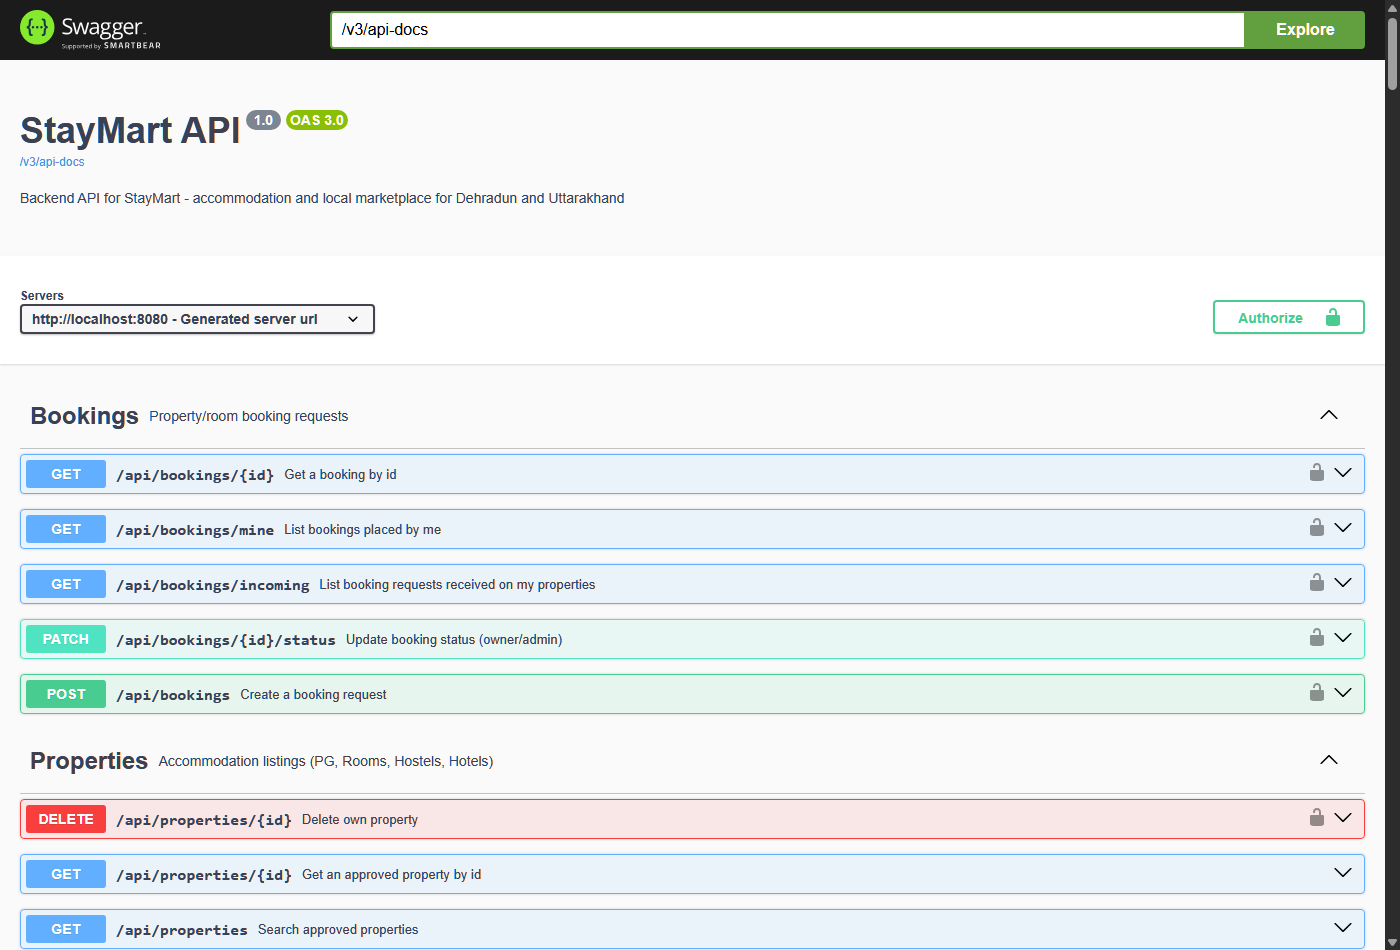
\includegraphics[width=0.95\textwidth]{screenshots/swagger_api.png}
    \caption{Springdoc OpenAPI 3.0 Swagger UI Exposing Core Backend REST Endpoints}
    \label{fig:swagger_api}
\end{figure}

The 16 REST controllers in \texttt{src/main/java/com/staymart/controller/} are organized into four functional groups:
\begin{enumerate}
    \item \textbf{Identity and Profile Management:} \texttt{AuthController} (registration and login), \texttt{UserController} (profile management and verification), and \texttt{FileController} (photograph asset uploads).
    \item \textbf{Accommodation and Inventory:} \texttt{PropertyController} (PG, hostel, and flat listings), \texttt{RoomController} (room configurations and capacities), and \texttt{LocationController} (Uttarakhand campus clusters).
    \item \textbf{Campus Classifieds:} \texttt{ProductController} (student gear listings for sale or rent) and \texttt{CategoryController} (marketplace taxonomy).
    \item \textbf{Interactions and Administration:} \texttt{BookingController} (accommodation reservations), \texttt{OrderController} (product acquisitions), \texttt{ChatController} (in-app student messaging), \texttt{ReviewController} (ratings and feedback), \texttt{WishlistController} (saved listings), \texttt{BehaviorController} (user telemetry events), \texttt{RecommendationController} (personalized and trending feeds), and \texttt{AdminController} (listing moderation and user management).
\end{enumerate}

\subsection{Standardized API Envelope Pattern}
To ensure client applications receive predictable payload structures regardless of success or failure states, all endpoints emit an \texttt{ApiResponse<T>} envelope:

\begin{lstlisting}[language=Java, caption={Generic API Response Wrapper}]
public class ApiResponse<T> {
    private boolean success;
    private String message;
    private T data;
    private Long timestamp;

    public static <T> ApiResponse<T> ok(T data) {
        return new ApiResponse<>(true, "Success", data, System.currentTimeMillis());
    }

    public static <T> ApiResponse<T> ok(String message, T data) {
        return new ApiResponse<>(true, message, data, System.currentTimeMillis());
    }

    public static <T> ApiResponse<T> error(String message) {
        return new ApiResponse<>(false, message, null, System.currentTimeMillis());
    }
}
\end{lstlisting}

Pagination responses encapsulate content lists alongside cursor metadata via \texttt{PageResponse<T>}:
\begin{lstlisting}[language=Java, caption={Paginated Response Wrapper}]
public record PageResponse<T>(
    List<T> content,
    int page,
    int size,
    long totalElements,
    int totalPages,
    boolean last
) {
    public static <T> PageResponse<T> from(Page<T> springPage) {
        return new PageResponse<>(
            springPage.getContent(),
            springPage.getNumber(),
            springPage.getSize(),
            springPage.getTotalElements(),
            springPage.getTotalPages(),
            springPage.isLast()
        );
    }
}
\end{lstlisting}

\section{Security Architecture: Spring Security and Stateless JWT}
Security in StayMart is managed by Spring Security 6, enforcing stateless authentication using JSON Web Tokens (JWT) to avoid server-side session overhead.

\subsection{JWT Signing and Roles}
Upon successful login via \texttt{POST /api/auth/login}, the \texttt{JwtTokenProvider} generates a signed token:
\begin{itemize}
    \item \textbf{Algorithm:} HMAC-SHA256 (\texttt{HS256}) using a 256-bit secret key.
    \item \textbf{Token Claims:} Subject (\texttt{email}), User ID (\texttt{id}), Role authority (\texttt{ROLE\_USER} or \texttt{ROLE\_ADMIN}), Issue time (\texttt{iat}), and Expiration (\texttt{exp}, 24 hours).
\end{itemize}

\subsection{JWT Authentication Filter}
Every inbound HTTP request passes through \texttt{JwtAuthenticationFilter} before reaching the servlet dispatcher:

\begin{lstlisting}[language=Java, caption={JwtAuthenticationFilter Request Interceptor}]
@Component
public class JwtAuthenticationFilter extends OncePerRequestFilter {

    private final JwtTokenProvider tokenProvider;
    private final CustomUserDetailsService userDetailsService;

    @Override
    protected void doFilterInternal(HttpServletRequest request,
                                    HttpServletResponse response,
                                    FilterChain filterChain) throws ServletException, IOException {
        String token = resolveToken(request);
        if (StringUtils.hasText(token) && tokenProvider.validateToken(token)) {
            String email = tokenProvider.getEmailFromToken(token);
            UserDetails userDetails = userDetailsService.loadUserByUsername(email);
            
            UsernamePasswordAuthenticationToken authentication =
                new UsernamePasswordAuthenticationToken(userDetails, null, userDetails.getAuthorities());
            authentication.setDetails(new WebAuthenticationDetailsSource().buildDetails(request));
            
            SecurityContextHolder.getContext().setAuthentication(authentication);
        }
        filterChain.doFilter(request, response);
    }

    private String resolveToken(HttpServletRequest request) {
        String bearer = request.getHeader("Authorization");
        if (StringUtils.hasText(bearer) && bearer.startsWith("Bearer ")) {
            return bearer.substring(7);
        }
        return null;
    }
}
\end{lstlisting}

\subsection{Accurate Security Boundaries}
Each security concern is handled at the appropriate architectural layer:
\begin{itemize}
    \item \textbf{Password Encryption:} Passwords are encrypted with BCrypt ($cost=10$) before database persistence.
    \item \textbf{Authentication and RBAC:} JWT tokens provide stateless session verification and role enforcement. Standard users have access to personal bookings, chats, and listings, while admin routes require \texttt{ROLE\_ADMIN}.
    \item \textbf{SQL Injection Defense:} Provided by Spring Data JPA and Hibernate ORM parameterized queries (\texttt{PreparedStatements}), which treat user inputs strictly as literal parameters.
    \item \textbf{XSS Defense:} Handled by frontend output sanitization via \texttt{escapeHtml()} in \texttt{utils.js} and input validation annotations in Spring Boot DTOs.
\end{itemize}

\section{Machine Learning Recommendation Microservice}
The recommendation microservice is implemented in Python 3.11 with Flask in \texttt{ml-service/}, using scikit-learn for TF-IDF vector transformations.

\subsection{Feature Vectorization and Model Pipeline}
For each listing, the service synthesizes a composite text document concatenating title, description, category, campus area, city, amenities, and price tier buckets:

\begin{lstlisting}[language=Python, caption={Property Text Document Synthesis in recommender.py}]
def build_property_document(row):
    tokens = [
        str(row['title']),
        str(row['description']),
        str(row['type']),
        str(row['gender_preference']),
        str(row['area']),
        str(row['city']),
        " ".join(json.loads(row['amenities'])) if row['amenities'] else ""
    ]
    price = float(row['price_per_month'])
    if price < 5000:
        tokens.append("budget_tier_low")
    elif price <= 10000:
        tokens.append("budget_tier_medium")
    else:
        tokens.append("budget_tier_premium")
    return " ".join(tokens)
\end{lstlisting}

The composite corpus is transformed into a continuous vector space using \texttt{TfidfVectorizer} with unigrams and bigrams $(1, 2)$, sublinear term frequency scaling, and English stop-word filtering. Cosine similarity calculates relevance scores:
\begin{equation}
\text{Similarity}(\vec{u}, \vec{v}) = \frac{\vec{u} \cdot \vec{v}}{\|\vec{u}\|_2 \|\vec{v}\|_2}
\end{equation}

\begin{figure}[htbp]
    \centering
    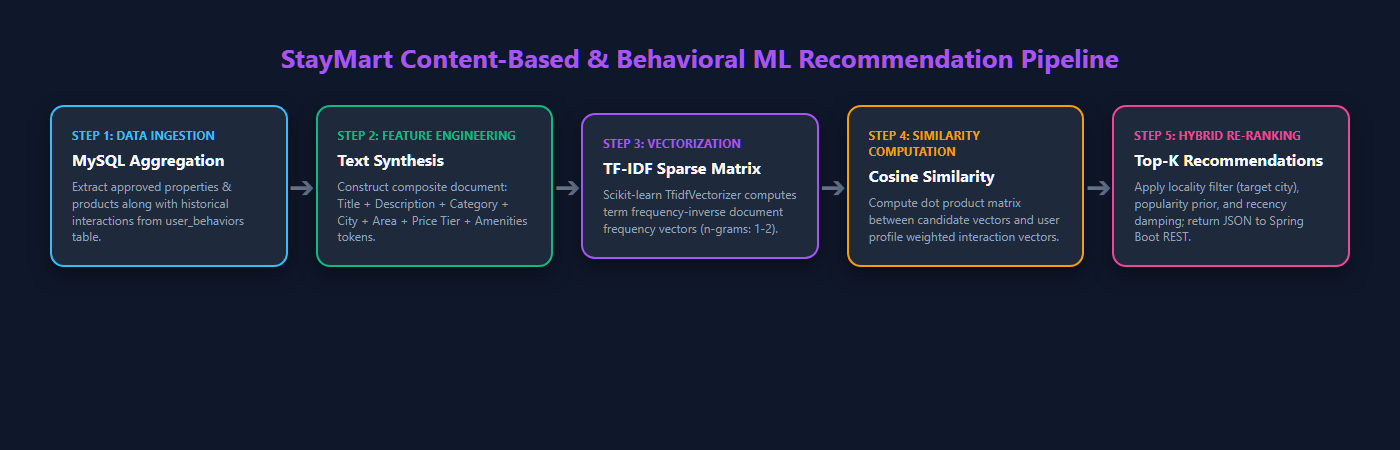
\includegraphics[width=0.92\textwidth]{diagrams/ml_pipeline.png}
    \caption{Machine Learning Content-Based Recommendation Pipeline with TF-IDF Vectorization}
    \label{fig:ml_pipeline}
\end{figure}

\section{Fault-Tolerant Fallback Integration in Spring Boot}
The Spring Boot backend interacts with the Flask ML microservice through \texttt{MlServiceClient}. To ensure platform availability when the ML service is offline or starting up, \texttt{MlServiceClient} configures a 2000ms connection timeout and a 3000ms read timeout:

\begin{lstlisting}[language=Java, caption={Timeout Configuration in MlServiceClient.java}]
SimpleClientHttpRequestFactory requestFactory = new SimpleClientHttpRequestFactory();
requestFactory.setConnectTimeout(2000); // 2000ms connect timeout
requestFactory.setReadTimeout(3000);    // 3000ms read timeout
this.client = builder.baseUrl(mlBaseUrl).requestFactory(requestFactory).build();
\end{lstlisting}

If the ML microservice throws a \texttt{RestClientException} or returns an unparseable response, \texttt{MlServiceClient} catches the exception, logs a warning, and returns an empty list.

The \texttt{RecommendationService} detects this empty list and immediately falls back to approved database listings:

\begin{lstlisting}[language=Java, caption={Resilient Database Fallback in RecommendationService.java}]
@Service
public class RecommendationService {

    private final MlServiceClient mlServiceClient;
    private final PropertyService propertyService;
    private final ProductService productService;

    public List<PropertyResponse> recommendedProperties(Long userId, String city, int limit) {
        List<Long> ids = mlServiceClient.fetchRecommendedPropertyIds(userId, resolveCity(city), limit);
        List<PropertyResponse> properties = ids.isEmpty()
                ? List.of()
                : propertyService.findRecommendedProperties(ids, limit);
        if (properties.isEmpty()) {
            return propertyService.latestApproved(limit); // Resilient JPA fallback
        }
        return properties;
    }
}
\end{lstlisting}

This design guarantees that even if the Python ML microservice is unavailable, students browsing StayMart continue to receive valid, verified listings without encountering HTTP 500 errors.

\section{Summary}
This chapter detailed the backend and machine learning implementation of StayMart. We analyzed the Controller-Service-Repository architecture across 16 REST controllers, stateless JWT security, and data validation rules in Spring Boot 3.3 under Java 17 LTS. We documented the TF-IDF feature vectorization pipeline and the resilient database fallback mechanism in \texttt{RecommendationService}. The next chapter explores the frontend UI/UX design system and client-side JavaScript architecture.
